% !TEX root = ../thesis.tex

\chapter{Previous Work}\label{cha:prev}
This chapter provides an overview of what my workings on the initial \gls{CPU} included.

\section{Design Goal}
My initial goal was to design a \gls{CPU} from scratch without explicitly looking at how other architectures had solved occurring problems.
This meant I was to rely on the knowledge I had achieved until then and came up with the following specifications I wanted my \gls{CPU} to fulfill:
\paragraph{8 bit bus width}
Most current era \glspl{CPU} employ a 32 bit or 64 bit bus to handle large numbers and large amounts of data.
It was clear to me that I needed to settle for a smaller bus when building a \gls{CPU} by hand.
Some early \glspl{CPU} worked with only 4 bits but to not be as limited I finally chose to use an 8 bit bus.
\paragraph{Datapath Architecture - Multicycle CISC}
In most \glspl{CPU} an instruction is not done in one clock cycle but it is divided into several steps that are done in sequence.
There are two general approaches that are called \emph{Multicycle} and \emph{Pipelining} \cite{PattersonDavid2016RuRD}.
Multicycle means that all the steps of one instruction are performed sequentially and a new instruction is only dispatched after the previous instruction is finished.
This is usually used when implementing \glspl{CISC}, where one instruction can be very capable \cite{chen_novick_shimano_2000}.
For example a add instruction in \gls{CISC} could fetch operands from memory, execute the add and write the result back to memory.
\glspl{RISC} on the other hand would need independent instruction to load operands from memory into registers, do the addition and write the result back to memory.

In Pipelining there a fixed steps each instruction goes through in a defined order and the intermediate results are stored in so called pipeline registers.
Each pipeline step is constructed in such a way that it does not intervene with the others.
Therefore, it is possible to dispatch a new instruction each cycle even though the previous instruction is not yet finished.
A typically 5-step pipeline would consist of the following steps \cite{PattersonDavid2016RuRD}:
\begin{enumerate}
  \item \textbf{Instruction Fetch}: The instruction is retrieved from memory and stored in a register.
  \item \textbf{Instruction Decode}: The fetched instruction is decoded into control signals (and instruction specific data) for all the components of the \gls{CPU}.
  \item \textbf{Execute}: If arithmetic or logical operations are part of the instruction, they are performed.
  \item \textbf{Memory Access}: Results are written to the memory and/or data is read from memory.
  \item \textbf{Writeback}: The results are written back to the registers.
\end{enumerate}
However good the performance of a pipelined \gls{CPU} is, it also comes with challenges.
Those include a greater resource usage because all intermediate results need to be stored in pipeline registers.
Additionally, branch instructions\footnote{Branch Instructions change the \gls{PC} and with that the location from which the next instruction is to be fetched. This is required for conditional and looped execution.} pose a great challenge because at the moment, the \gls{CPU} execute the branch the next instructions have already been dispatched.
This means that the pipeline needs to be flushed (i.e. cleared), performance is lost and more logic is required.
It also noteworthy that branch prediction and pipeline flushes can be quite vulnerable as recently shown in CVE-2017-5753 with the Spectre bug \cite{CVE-2017-5753}.

Therefore, I decided to build my \gls{CPU} as a Multicycle \gls{CISC}.

\paragraph{Single-Bus Oriented}
The decision for a Multicycle \gls{CPU} also enabled the architecture to be single-bus oriented.
This means that all modules (e.g. the \gls{ALU} and the memory) are connected to a central bus for data transfer.
The central bus is then used as a multi-directional data communication.
To allow this in hardware, all components that drive the bus (i.e. ``send'' data) need to have a tri-state driver.
A tri-state driver can either drive the bus with a defined `0' or `1' or high impedance which allows other tri-state drivers on the same bus to drive it.
That way an instruction which fetches a word from the memory from an address stored in a register and stores it in a register could consist of the following steps:
\begin{enumerate}
  \item Instruction Fetch
  \item Instruction Decode
  \item Memory Address from register over \emph{bus} to memory module
  \item Memory Access
  \item Data from memory module over \emph{bus} to register
\end{enumerate}
With such an architecture it is possible to avoid large multiplexers and keep the overall architecture simple.

\section{Implementation}
As mentioned above, the \gls{CPU} is divided into multiple modules which are only connected over the bus apart from control signals and one other exception.
\subsection{Modules}
The original design was split into 7 independent modules of varying complexity.
\subsubsection{\glsxtrfull{ALU}}
\begin{table}
  \centering
  \renewcommand{\arraystretch}{1.25}
  \caption{Summary of the available alu operations.}
  \label{tab:aluOp}
  \begin{tabularx}{.8\textwidth}{ |c|c|c||X| }
    \hline
    aluOp[1] & aluOp[0] & aluSub & Resulting Operation             \\\hline\hline
    0        & 0        & 0      & ($A + B$) Addition              \\\hline
    0        & 0        & 1      & ($A - B$) Subtraction           \\\hline
    0        & 1        & 0      & ($A \land B$) AND               \\\hline
    0        & 1        & 1      & ($A \land \overline{B}$)        \\\hline
    1        & 0        & 0      & ($A \veebar B$) XOR             \\\hline
    1        & 0        & 1      & ($\overline{A \veebar B}$) XNOR \\\hline
    1        & 1        & 0      & ($A \gg B$) logical shift right \\\hline
    1        & 1        & 1      & ($A \ll B$) logical shift left  \\\hline
  \end{tabularx}
\end{table}
The \gls{ALU} is capable of 4 different operations plus inverting the $B$ input for two's complement subtraction.
Therefore, there are three control signals which control the operation: two alu-operation bits plus one subtract bit.
The $B$ input is XORed with the aluSub bit which results in the $B$ input being inverted when aluSub is `1' and otherwise $B$ remains the same.
The aluSub bit is also connected to the carry input of the adder and with that, results in a two's complement subtraction.
All possible operations are shown in \cref{tab:aluOp}.
\begin{figure}[t]
  \centering
  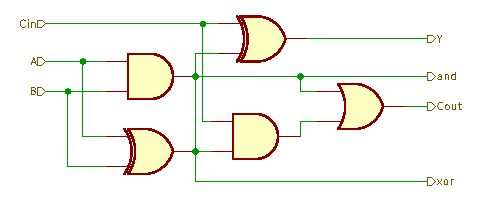
\includegraphics[width=\textwidth]{full_adder.pdf}
  \caption{1 bit full adder with the usual A, B and Carry inputs and Y and Carry outputs as well as the XOR and AND outputs.}
  \label{fig:full_adder}
\end{figure}
The adder is a simple ripple carry adder for its simplicity and the XOR and AND operation from the half-adders are also used as the logic operations.
A complete 1 bit full-adder is shown in \cref{fig:full_adder}.

\begin{sidewaysfigure}[p]
  \centering
  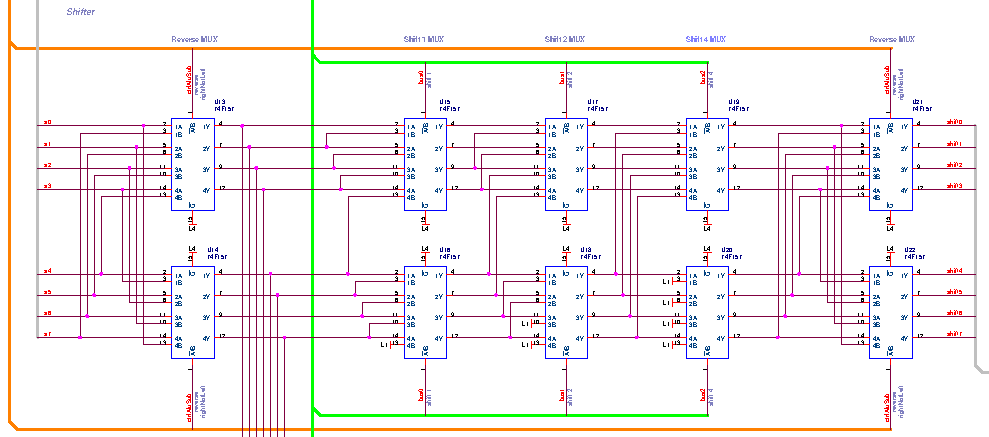
\includegraphics[width=\linewidth]{barrel_shifter.pdf}
  \caption{8 bit bidirectional barrel shifter.}
  \label{fig:barrel_shifter}
\end{sidewaysfigure}
It was desirable to include a barrel shifter to have the possibility to improve multiply operation with a shift and add approach instead of repeated addition.
The barrel shifter works by 3 consecutive multiplexers to shift by 1, 2 or 4 bit to the right that are controlled by the first 3 bit of the (not inverted) $B$ input.
To also allow shifting to the left there is one multiplexer before the three shift multiplexers to invert the order of bits and another one after the shifting to reorder the bits.
In \cref{fig:barrel_shifter} a bidirectional barrel shifter implemented with the \texttt{74F157} is visualized. The \texttt{74F157} implements four 2 to 1 multiplexer and, therefore, 2 chips are needed for a full 8 bit 2 to 1 multiplexer.

The multiplexed result is stored in an 8 bit \gls{ALU} result register.
For conditional execution the \gls{ALU} includes two flags: Not Zero (at least one bit is one) and negative (the \gls{MSB}).

\subsubsection{Register File}
As is typical with \glspl{CISC} the \gls{CPU} does not need many general purpose registers and the register file can be kept simple with only two registers.
The register file has one write port (from the bus) and two read ports of which one reads to the bus and the other is directly connected to the $A$ input of the \gls{ALU}.
\subsubsection{Control Logic}\label{ssec:cl}
The control logic's job is to decode the current instruction and provide all the control signals for each cycle for any instruction.
For keeping track which cycle of each instruction is currently executing a 3 bit synchronous counter is needed.
Each control signal could be derived by a logical circuitry with 13 inputs: 8 bits instruction, 2 bits \gls{ALU} flags and 3 bits cycle counter.
However, designing these logic circuits is a lot of work, takes up a lot of space and cannot be changed easily later on. (For example when finding a bug in one instruction)
Therefore, an \gls{EEPROM} is used where the 13 bits that define one cycle of one specific instruction are used as addresses.
The control signals then are the data bits of the word that is stored at the specific address in the \gls{EEPROM}.

The first two cycles of each instruction need to be taken in special consideration because the instruction register is not yet loaded with the next instruction, because it is still being fetched and decoded.
However, the instruction fetch and decode are always the same for each instruction, which means that all memory locations where the cycle counter is equal to 0 or 1 (the first two instructions) are filled with the control signals for an instruction fetch and decode.
\subsubsection{Memory}
The memory module contains the main memory of the \gls{CPU} in form of an asynchronous \gls{SRAM} and the instruction memory as an \gls{EEPROM}.
This way a new program can be loaded into the \gls{CPU} by reprogramming the \gls{EEPROM}.
Both the \gls{SRAM} and the \gls{EEPROM} have their data lanes connected to the bus for reading from and writing to the memory.
The address is controlled via an \gls{MAR} from the bus.
\subsubsection{\glsxtrfull{PC}}
The \gls{PC} is a special register with two main functionalities:\\
Usually it increments by one after each instruction.
However, when a branch is executed it needs to load the branch address from the bus.
For this an 8 bit increment similar to the cycle counter from the Control Logic \cref{ssec:cl} is multiplexed with the bus and used as the input data for the register.
\subsubsection{Input \& Output}
This first version of the \gls{CPU} included very rudimentary I/O logic.
For input it provides an 8 bit DIP-Switch connected to the bus and for output there is a register with a 2 digit 7-segment display.
\subsubsection{Clock \& Reset}
The function of the clock module is threefold:\\
It provides a clock for the whole \gls{CPU} while also providing an active-low reset for some of the registers to provide a defined starting condition.
The clock has two modes. One to run continuously and another where the clock can be manually advanced.
Additionally, there is a halt instruction which stops the \gls{CPU} clock until a button is pressed.
\subsection{FPGA Simulation}
The goal of the \gls{FPGA} simulation is to proof the general workings of the \gls{CPU} architecture.
There was no attempt made to provide a chip-level simulation of the hardware build but rather to provide a top-level behavioral model.
The chosen development environment is the AMD - Xilinx Vivado \cite{vivado} as it is freely available and provides an advanced simulation environment while providing the possibility to synthesize for relatively cheap \glspl{FPGA}.

One major problem with tri-state bus logic for \glspl{FPGA} is that most current era \glspl{FPGA} do not feature tri-state bus drivers in the logic.
Most \glspl{FPGA} do have bidirectional tri-state transceiver for I/O logic but not for internal logic routing.
However, the \glspl{HDL} (both \gls{VHDL} and Verilog) support tri-state logic and the Xilinx Simulation tool also does.
As the first \gls{CPU} was only simulated, this was not a problem and the tri-state logic could be used the same way as in the hardware build.
\Cref{cha:fpga} describes how tri-state logic is solved for the synthesis of the \gls{EDiC}.

\subsubsection{Language Choice}
There are two main \glspl{HDL}: Verilog and \gls{VHDL}.
Both are widely supported and used and can also be used in parallel in the same design.
At the \gls{TUB} \gls{VHDL} is taught and in Germany it also used more often.
However, in general both are used about equally often \cite{vhdlVerilog}.

As I only knew \gls{VHDL} and very basic concepts of Verilog, I decided to start in Verilog to get to know the differences.
\begin{listing}
  \inputminted[linenos,
    breaklines,
    firstline=24,
    lastline=61,
    % firstnumber=1,
    frame=leftline,
    xleftmargin=20pt,
  ]{verilog}{src/alu_proto.sv}
  \caption{(System)-Verilog Code for the \gls{ALU} of the first \gls{CPU} version.}
  \label{lst:alu_proto}
\end{listing}
\Cref{lst:alu_proto} shows the Verilog Code for the \gls{ALU} module (without the module definition to fit on one page).
Lines 24-28 describe the synchronous, positive-edge-triggered alu output register with a write enable.
The 8 XOR for the B input are described by lines 39-42 and lines 44-61 show an combinatorial process for the alu operation and multiplexing.
The lines 50-58 describe the bidirectional barrel shifter with 3 shift steps (by 1, 2, and 4) and the reverse \glspl{MUX} in front and at the end.
\subsection{Hardware Build}
The idea is to use \glspl{IC} of the well known 74 series for the logic functionality.
Initially, it was planned to build the \gls{CPU} similar to the 8-bit CPU project by Ben Eater \cite{eater_cpu} out of breadboards.
However, breadboards make for great prototyping but are known for their not-ideal connectivity and wires can come loose quite easily.
Especially when using about 15 boards errors due to bad connections are prone to happen.
On the other side, the proper approach would be to design a \gls{PCB} for the \gls{CPU}.
I decided against it for two main reasons:\\
I had little to no experience designing \glspl{PCB}, from layouting to placing and routing.
Additionally, I never worked with the 74 series \glspl{IC} and wanted to work with them in an easier to change environment similar to breadboards.
Secondly, designing such a large \gls{PCB} would have been very costly compared to what my financial plans for this project were.

\begin{figure}[t]
  \centering
  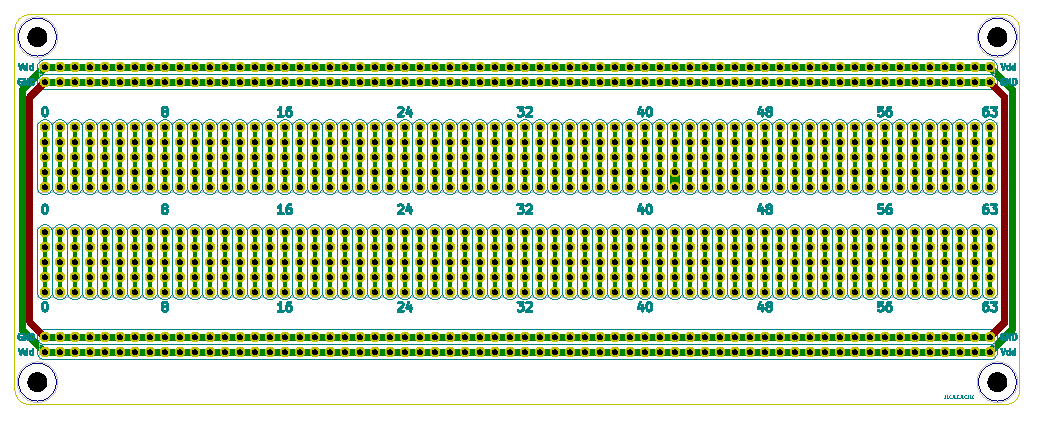
\includegraphics[width=\textwidth]{breadboardPcb.pdf}
  \caption{\gls{PCB} used for the hardware built of the first version of the \gls{CPU}.}
  \label{fig:breadboardPcb}
\end{figure}
Therefore, I decided to find a solution in the middle: A more permanent solution than breadboards but not already fully wired on a big \gls{PCB}.
I designed a small \gls{PCB} that is very similar to a breadboard with some minor tweaks to make it better suited for my goal.
It is shown in \cref{fig:breadboardPcb}.
I could order 25 of these boards from JLCPCB\footnote{\url{https://jlcpcb.com}} for only 34 USD shipped to Germany making it by far the cheapest option.

\begin{table}
  \centering
  \renewcommand{\arraystretch}{1.25}
  \caption{All logic \glspl{IC} used in the first \gls{CPU} version.}
  \label{tab:cpuIcs}
  \begin{tabularx}{\textwidth}{ |l|c||X| }
    \hline
    Quantity & \gls{IC}       & Function                                 \\\hline\hline
    23       & 74LS157        & quad 2 to 1 multiplexer                  \\\hline
    11       & 74LS08         & quad AND gate                            \\\hline
    9        & 74LS86         & quad XOR gate                            \\\hline
    6        & 74LS32         & quad OR gate                             \\\hline
    6        & 74LS374        & octal register (tri-state output)        \\\hline
    5        & 74LS245        & octal bus transceiver (tri-state output) \\\hline
    4        & 74LS273        & octal register with asynchronous clear   \\\hline
    4        & NA555P         & 555 timer                                \\\hline
    3        & 74LS00         & quad NAND gate                           \\\hline
    3        & 28C64          & 32k x 8 bit EEPROM (tri-state output)    \\\hline
    1        & AS6C1008-55PCN & 128k x 8 bit SRAM (tri-state output)     \\\hline
  \end{tabularx}
\end{table}
\begin{figure}[t]
  \centering
  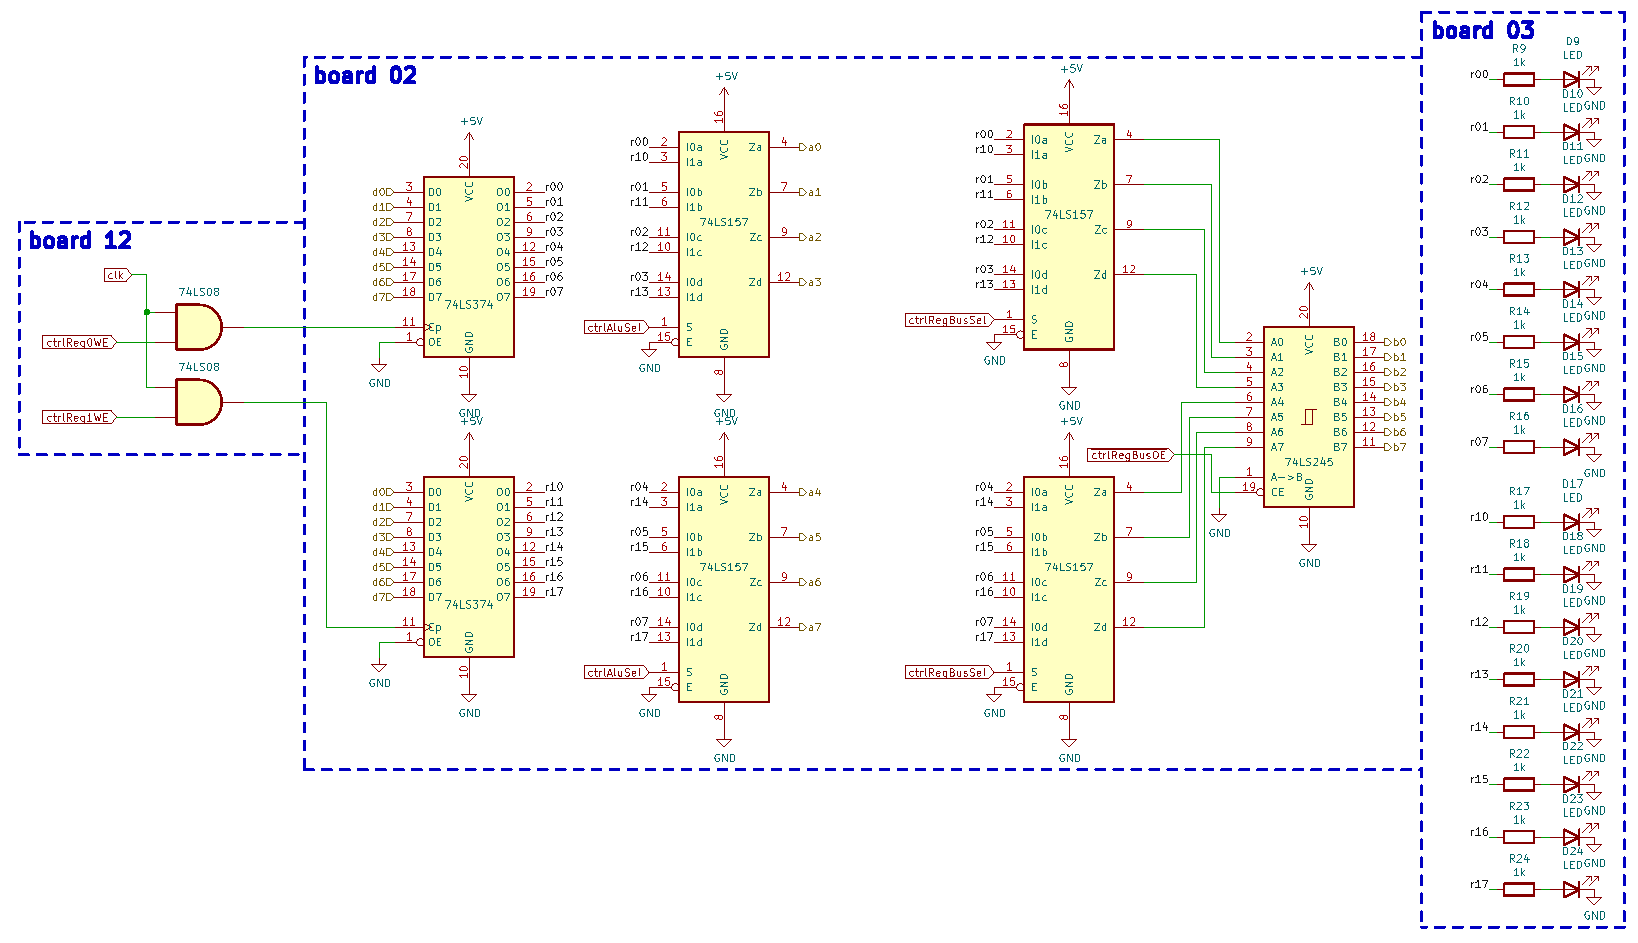
\includegraphics[width=\textwidth]{regset.pdf}
  \caption{Register File with two general purpose register, \gls{ALU} A input, bus driver and LEDs.}
  \label{fig:regset}
\end{figure}
The logic \glspl{IC} that have been used in the \gls{CPU} are listed in \cref{tab:cpuIcs}.
To make it easier to debug and also to visualize what the \gls{CPU} is calculating, most registers have \glspl{LED} attached to their outputs via resistors.
The layout of the register file is shown in \cref{fig:regset} as an example.
It can be seen that one breadboard-like \gls{PCB} holds 7 logic \glspl{IC} and the \glspl{LED} were placed on another board.
The clock pulse of the registers (\texttt{r0/1\_cp}) comes from another board where the clock has been ANDed with multiple \texttt{clockEnable} control signals (not all shown).
Problems of this kind of design and also how they were resolved for the \gls{EDiC} is presented in \cref{sec:improvements}.

\subsubsection{Clock Module}
\begin{figure}[t]
  \centering
  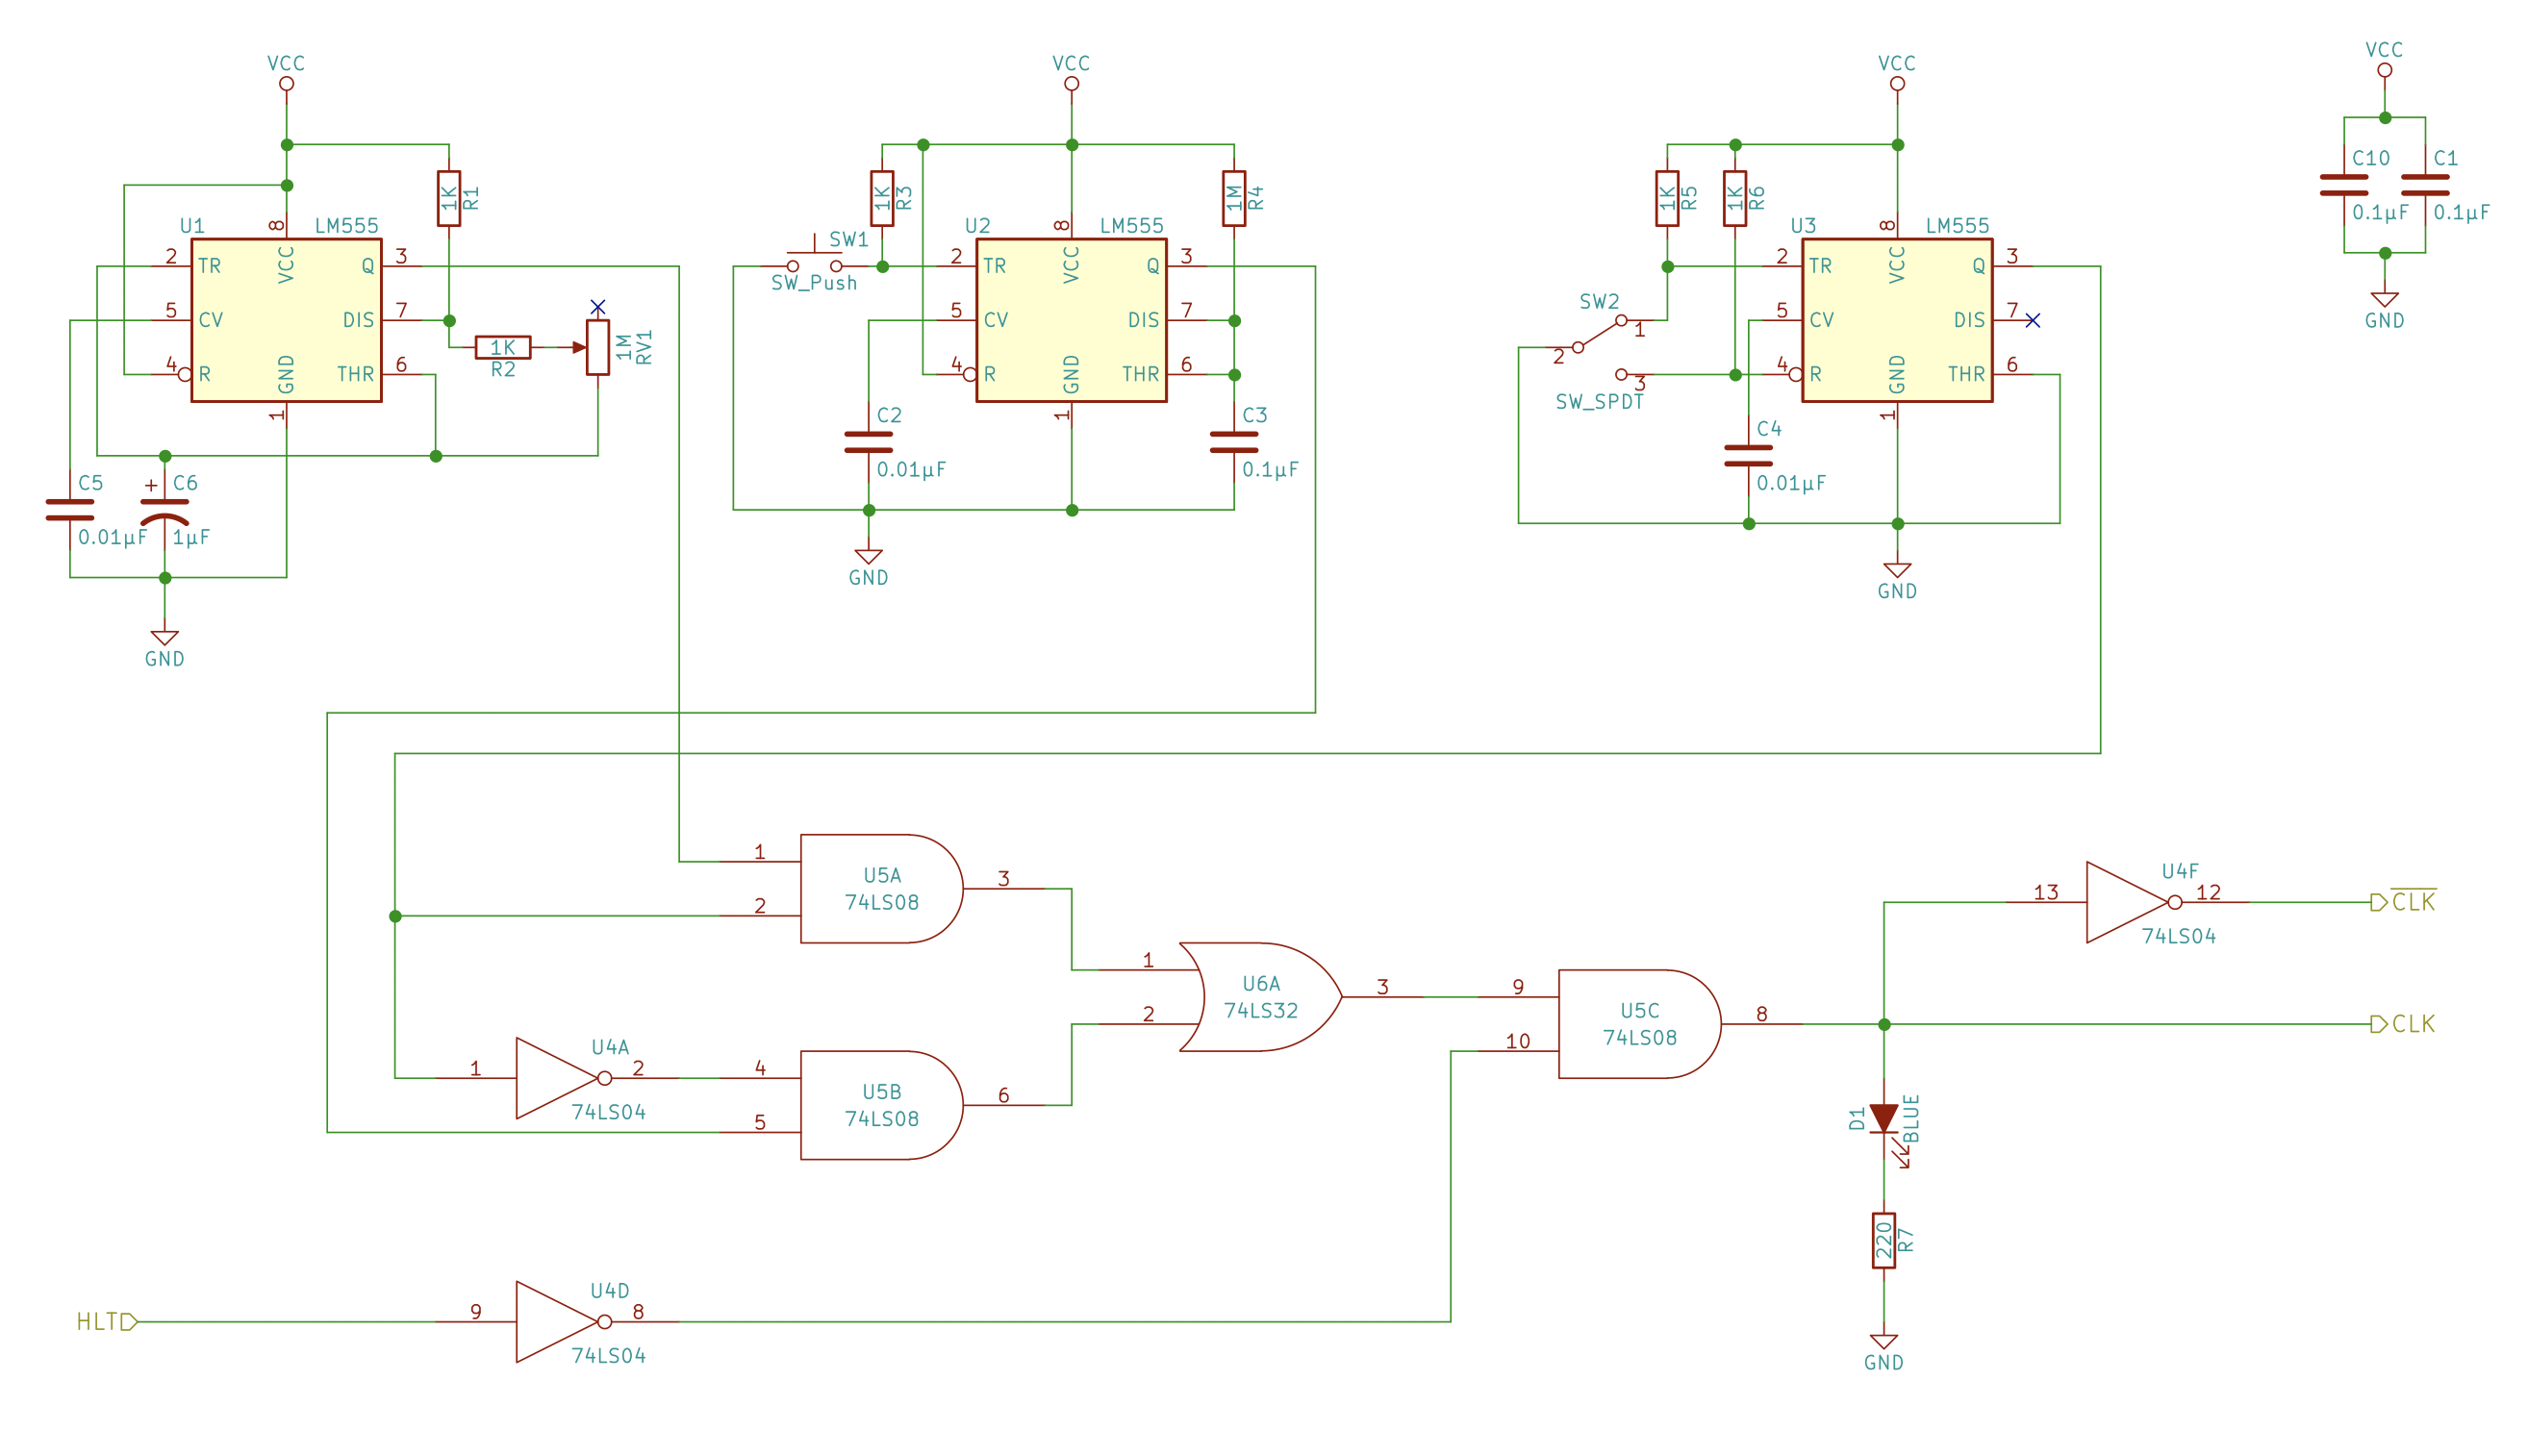
\includegraphics[width=\textwidth]{eater_clock.png}
  \caption{The schematic of the clock module by Ben Eater \cite{eater_clock} which inspired the clock module of the first version of the \gls{CPU}.}
  \label{fig:eater_clock}
\end{figure}
One clock module which cannot be simulated as well as the others is the clock module.
Its circuit is heavily inspired by the clock module of the above mentioned series by Ben Eater \cite{eater_clock} which exploits three possible use cases of the well known 555 timer.
The 555 timer \gls{IC} is a massively used \gls{IC} which features voltage dividers, two comparator, one SR flip-flop, an output driver and a discharge transistor \cite{LoweDoug555}.
As shown in \cref{fig:eater_clock} the three use cases for the 555 timer are in the astable (left), monostable (middle) and bistable (right) configuration.

The astable configuration works by charging C6 over R1, R2 and RV1 until a upper threshold voltage is reached which resets the internal flip-flop.
This allows the capacitor to discharge to the 555 internal ground until a lower threshold is reached and the flip-flop is set again to recharge the capacitor.
Depending on the capacitor and resistor dimensions this creates a never ending cycle of sets and resets of the flip-flop and in combination with the output buffer a clock.
By using a potentiometer as RV1 it is possible to control the clock frequency\footnote{The duty cycle of the clock is also affected but for the low frequencies I used this circuit (<1kHz) this has no effect on the logic circuit.}.

The monostable configuration is used to debounce a button press to be used for stepping the clock one cycle at a time.
It creates an active high pulse when the button is pressed once. All consecutive button presses (or bounces) only prolong the pulse but do not trigger another pulse.
If the button press would not be debounced it is possible that one press of the button results in multiple edges on the clock line which in turn can result in undefined and unknown behavior.
This was a cause for a small bug in the commissioning of the \gls{EDiC} as presented in \cref{sec:commissioning}.

The bistable configuration is used to switch between the two clock sources (astable and monostable).
It also uses the internal flip-flop to debounce the switch.

The lower logic gates are used to multiplex the two clock sources and additionally halt the clock when such an instruction is executed.
